\documentclass[12pt]{article}

\usepackage{setspace}
\usepackage{hyperref}
\usepackage{graphicx}
\usepackage{url}

\onehalfspacing

\parskip=2ex
\parindent=2em

\title{SWEN439 Visualisation Essay \\ John Snow's Cholera Map}
\author{Hai Tran 300224467}
\date{\today}

\begin{document}
\maketitle 

%Optional abstract
\begin{abstract}
This essay explores the famous visualisation created by John Snow to convince the general public that cholera epidemics were caused by water pumps. Through Snow's visualisation, it has influenced the field of GIS, thematic maps, and distributed dot maps. This essay looks into the history of the visualisation, the contribution of the visualisation, and how current research is explored to respect with the visualisation.

\end{abstract}

You will pick a visualisation and write an essay about that visualisation. 

You can do the cholera map, then show other things that were similar at the time, and for future show what visualisations came after that resemble it. Like dot maps. They would be not the main topic, but just an example of modern visualisations that are similar or you can contrast it with modern visualisations for disease spread to show how we do the same thing these days but use perhaps different visualisations.

\begin{itemize}
\item A clear description of the visualisation and how to read / interpret it
\item What questions does this visualisation address effectively and which does it not?
\item Is this a visualisation that is easy to use for novice viewers, or is it more intended for experts?
\item What is the history of the visualisation? Where did it come from? Where is / was it used?
\item What is the current state of research with respect to this visualisation?
\end{itemize}

\section{Introduction}

The essay explores an influential visualisation created by John Snow in the 18th century known as the Cholera Map. During that time, outbreaks of cholera - a deadly infectious disease that was thought to be spread via miasma, causing many deaths. The essay explores the history of the visualisation, how it came to be, the influence and contributions it had on the visualisation field, the questions that it addresses and does not address, and the current state of research with respect to the visualisation. In terms of the current state of research, the visualisation influenced the field of spot maps, and dot distributed maps. This essay will explore this area further in the essay.

\section{Snow's Cholera Map}

John Snow's Cholera Map consisted of a simple structure. Simple road maps were shown in his map to represent the area where he lived, Soho, London, England. Snow represented water pumps as black circles in his map, capitalising all the letters "PUMP". This enabled his intended audience to easily see the pump on the map. Snow recorded the people affected by the epidemic around his neighbourhood, tallying the deaths at each address. He represented each death at an address using horizontal bars. Each bar represented a death, multiple horizontally stacked bars represented multiple deaths. This enabled authorities to easily visualise the area in which most deaths occurred.  



\begin{figure}
\centering
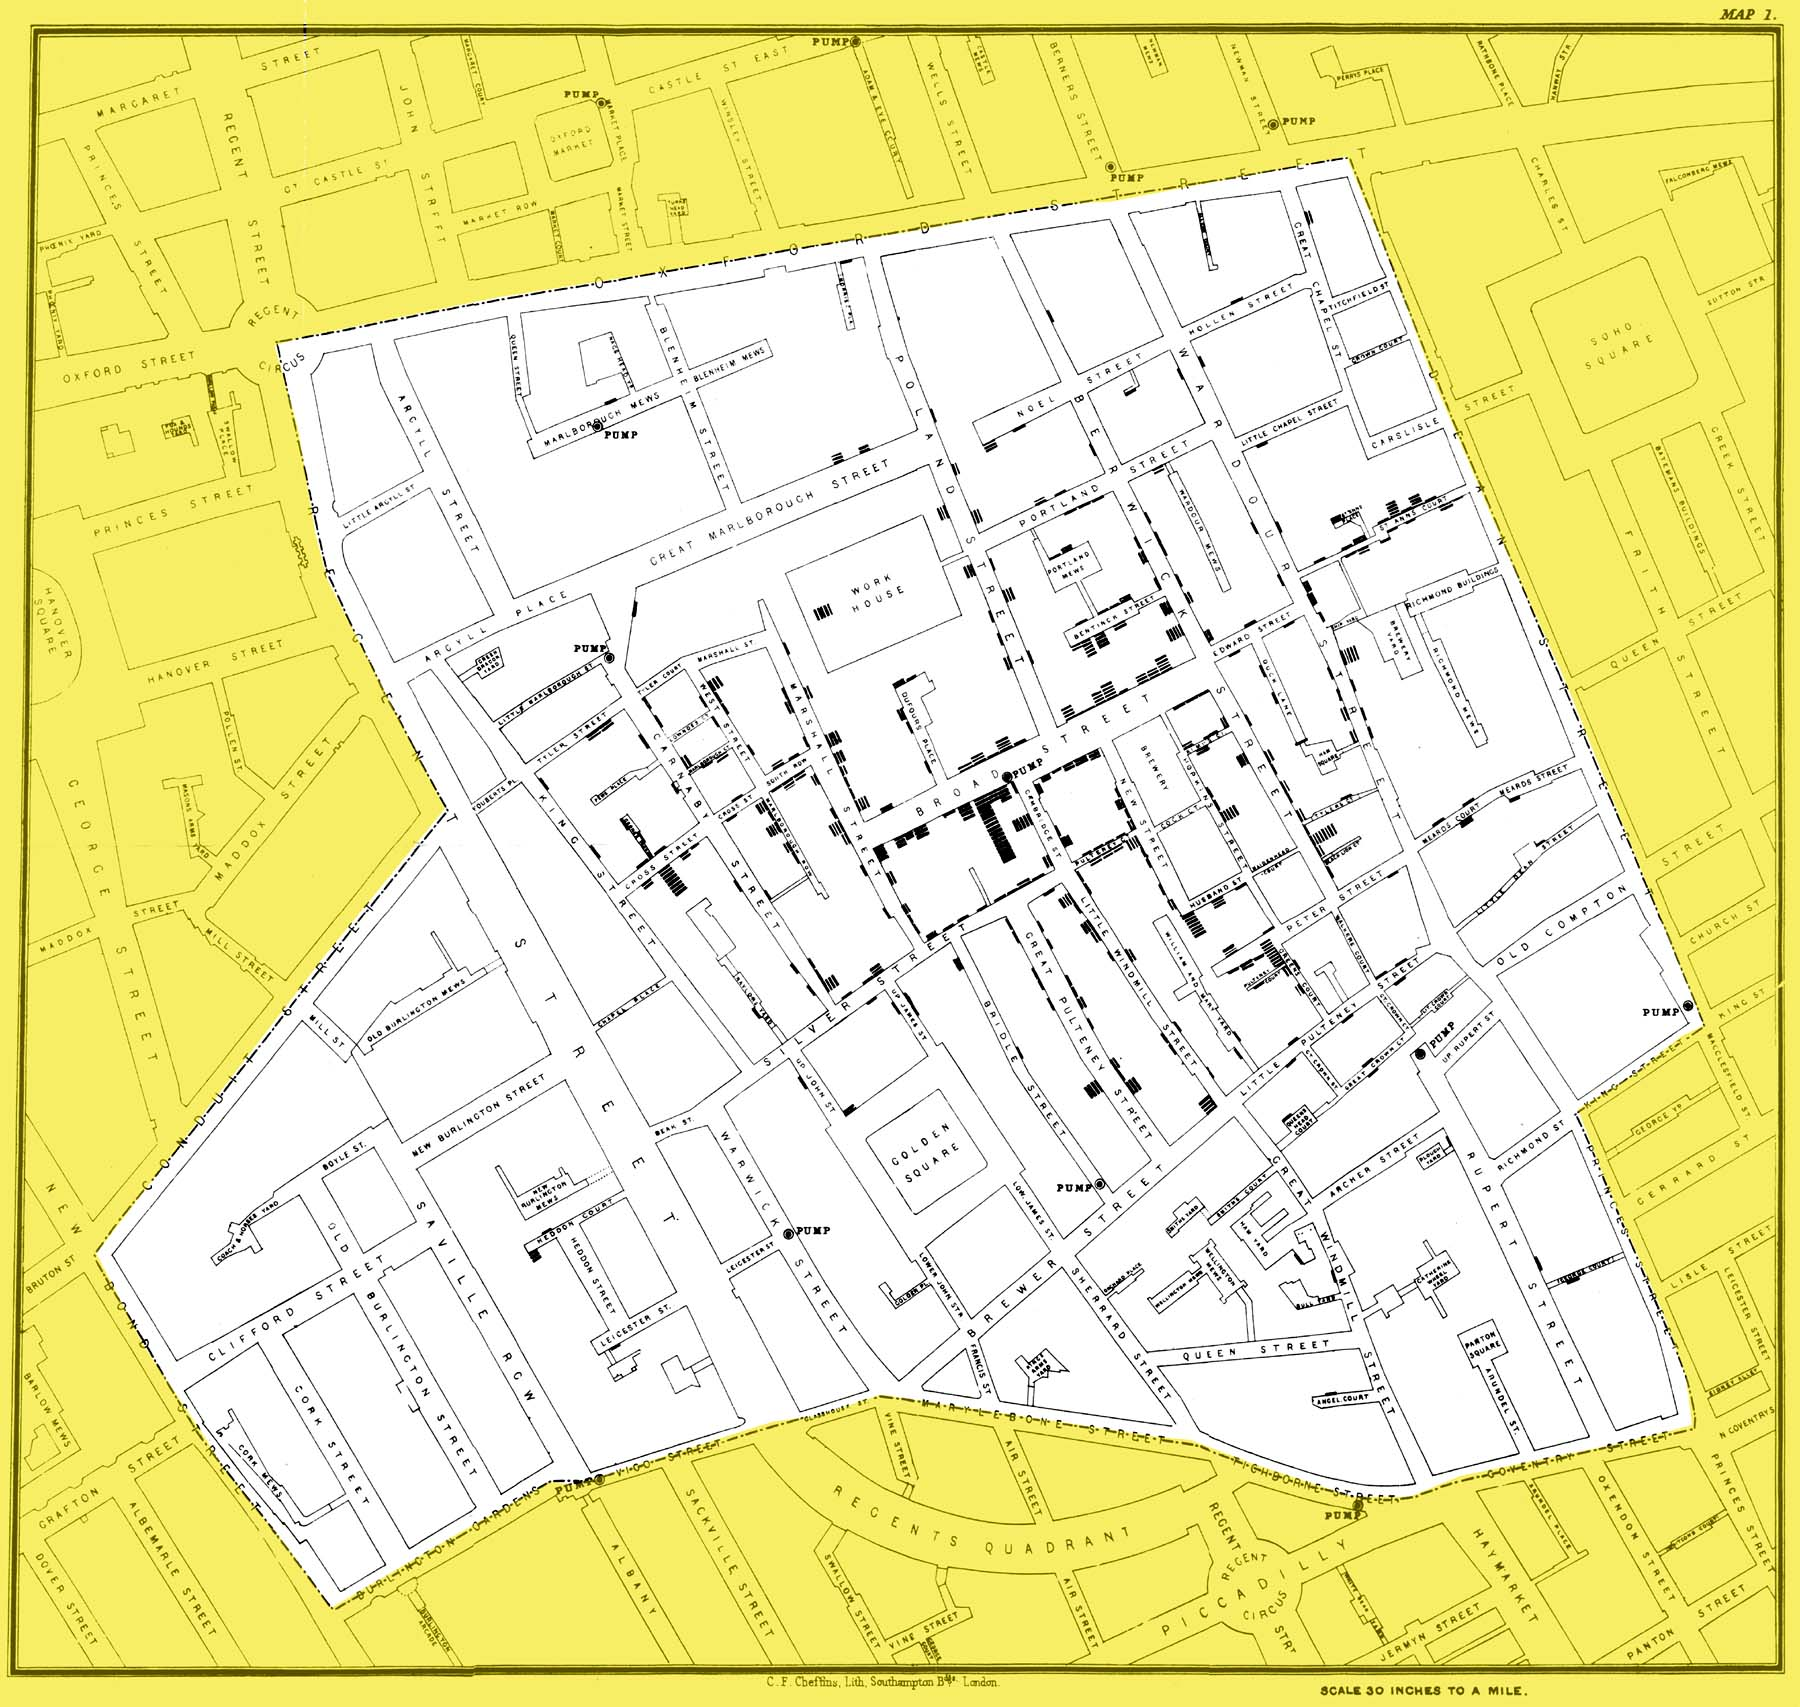
\includegraphics{snowmap_1854}
\caption{Caption}
\label{fig:snow}
\end{figure}

\begin{figure}
\centering
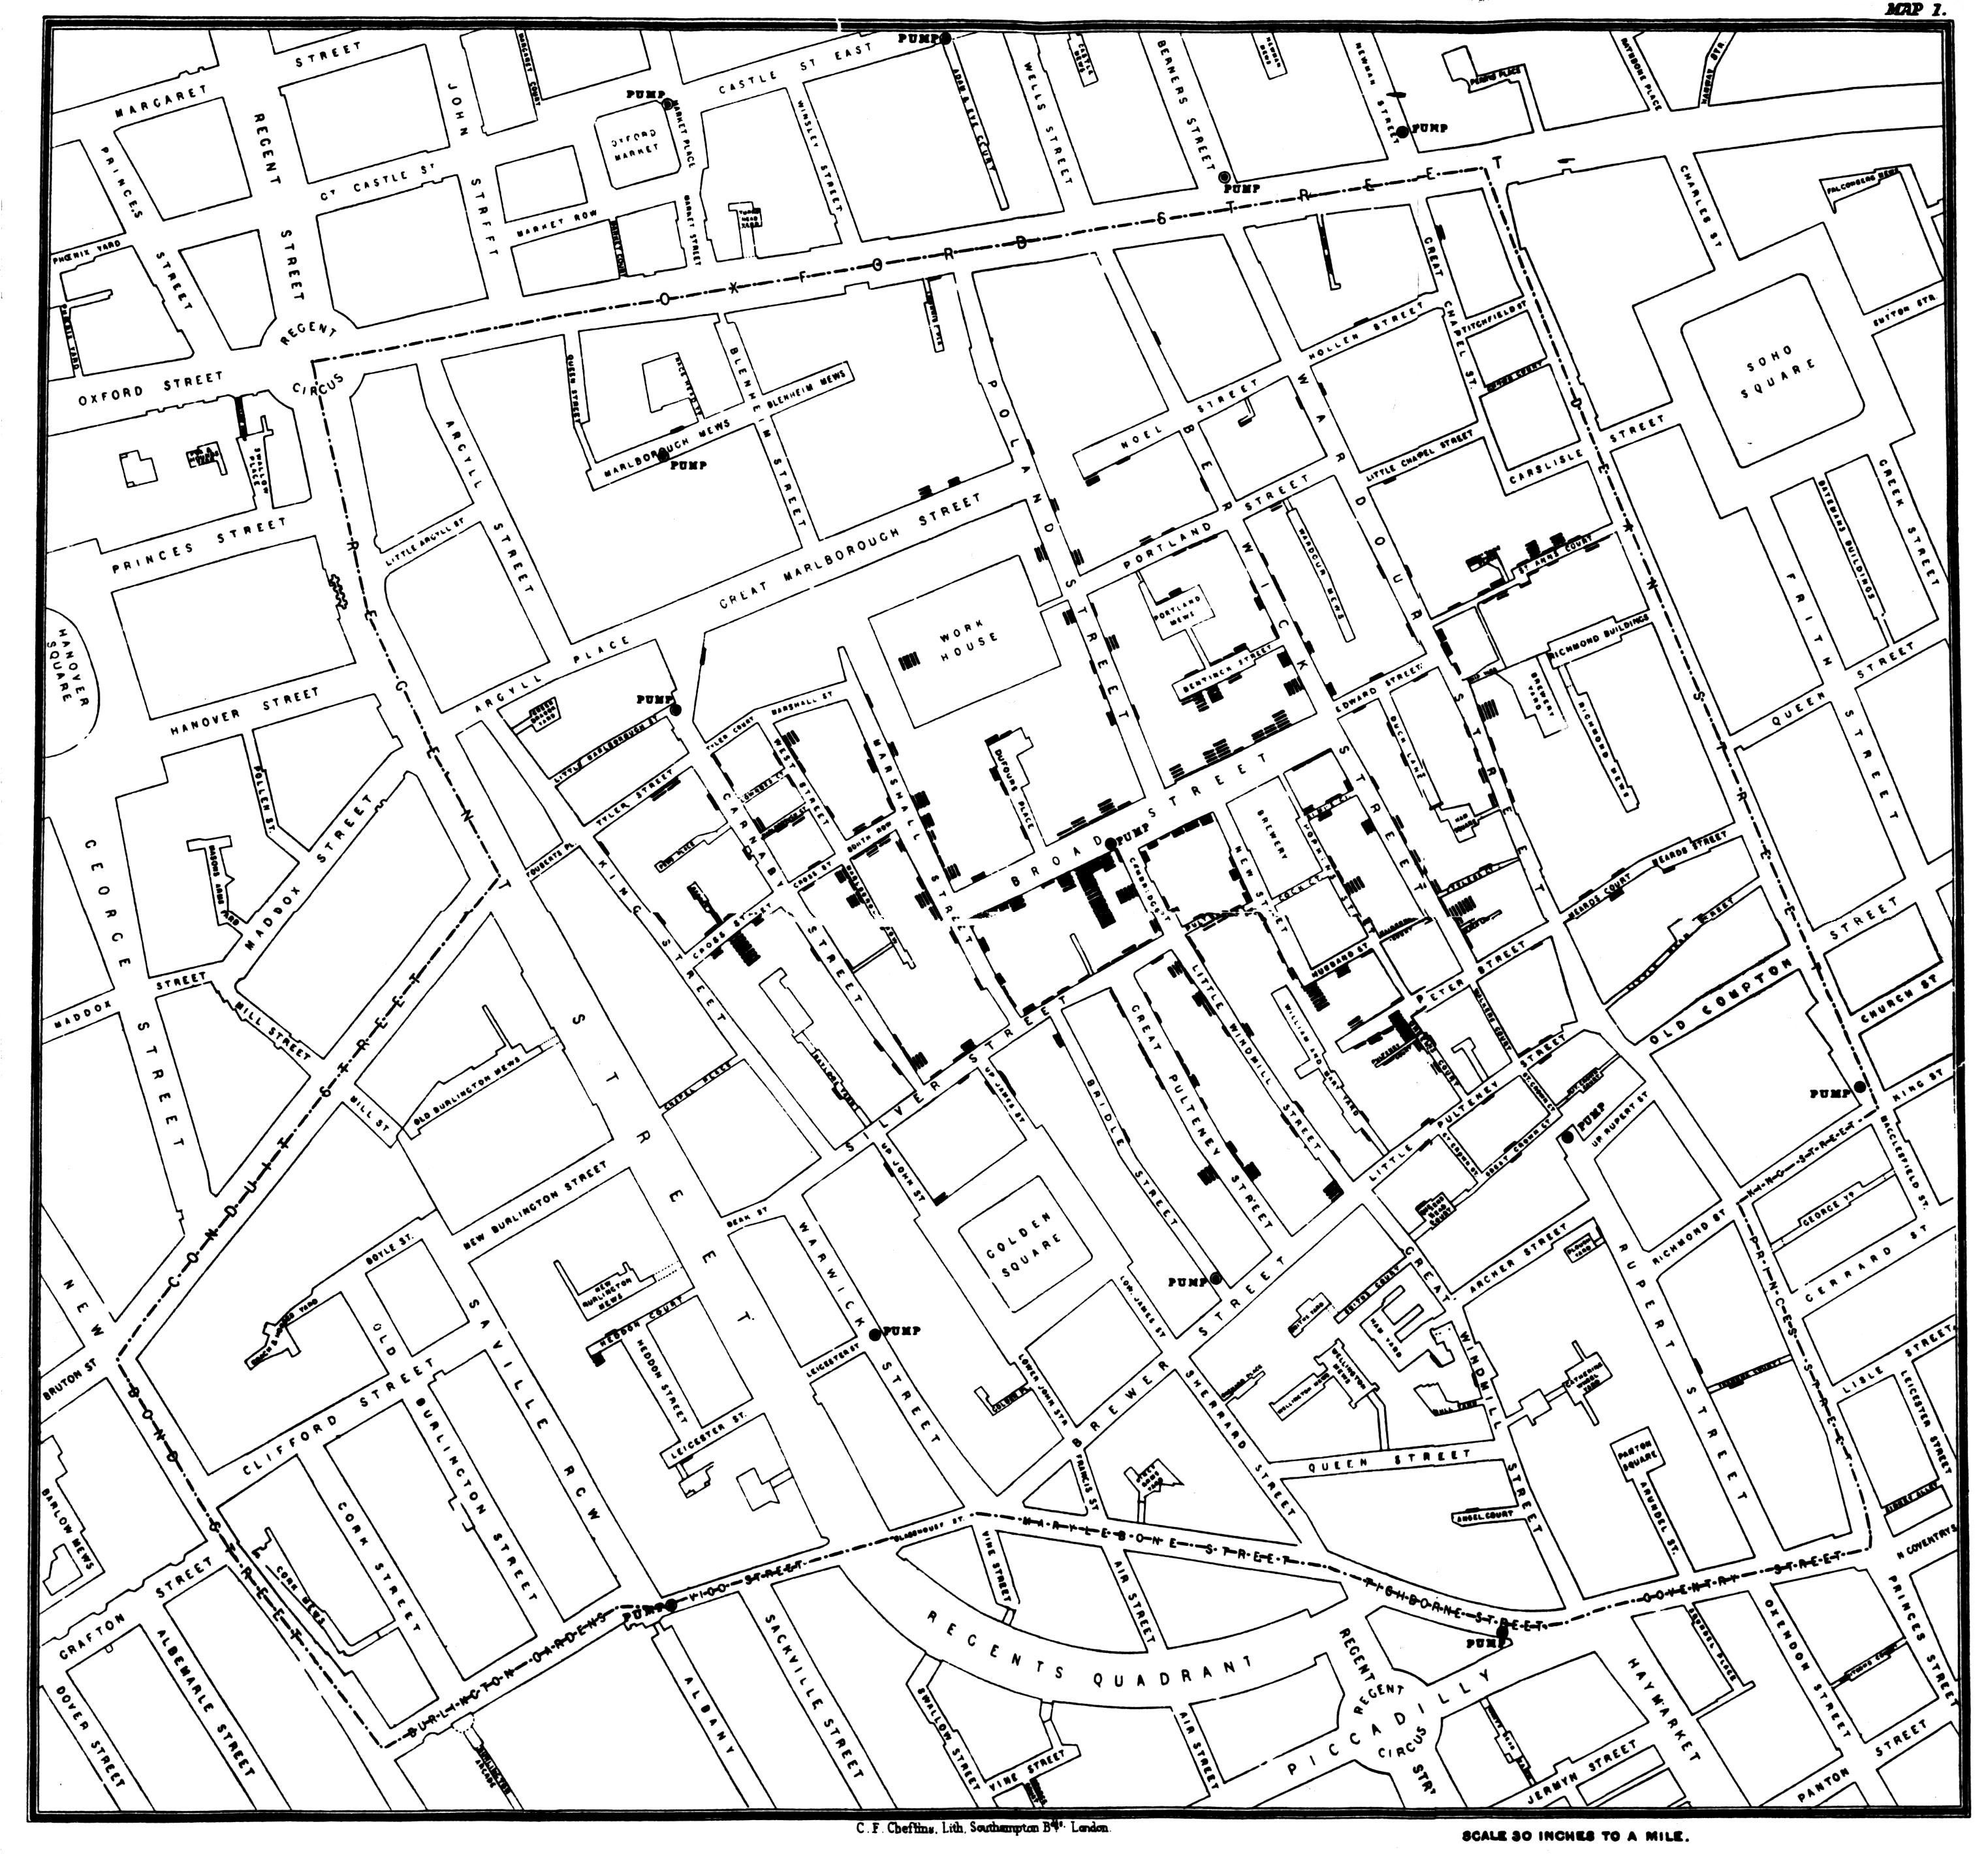
\includegraphics[scale=0.1]{Snow-cholera-map-1}
\caption{John Snow's Cholera map}
\label{fig:snow}
\end{figure}


\section{The Background of the Cholera Map}

Cholera outbreaks were known to appear around the 18th century. Cholera is a deadly disease that spreads through contaminated water and food sources. Aggressive vomiting occurs to victims, and they eventually die within 2 days. In the year 1854, the Broad Street cholera outbreak occurred in Soho district of London, England. It was known that around 500 civilians died due to the cholera. During this time, locals thought that cholera was a airborne disease that spread to anyone that comes in contact with the contaminated area. This led to many people fleeing the region during these times of outbreaks. However, a man called John Snow was a skeptic of the miasma theory and did not believe that cholera was an airborne disease caused by "bad air". Instead, Snow believed that cholera was spread through water. Snow, living around this region was able to record the resulting deaths around the neighbourhood to test his hypothesis. Although Snow had previously written several papers regarding Cholera and his hypothesis on the matter, no one believed Snow. After the epidemic, in order to raise awareness and to prevent anymore epidemics from occurring, Snow decided to plot the deaths from around the region on his map. Snow recorded each death as a horizontal bar, stacking multiple horizontal bars together at each address where a death occurred due to the epidemic that had previously occurred. Snow found that his visualisation showed deaths clustered around a water source, giving confidence in his hypothesis. The water source was a pump located on the Broad Street, where most of the highest frequency of deaths occurred. Snow warned authorities and tried to get the tap from the water pump removed. Eventually, authorities removed the water pump and the number of cholera victims decreased dramatically. 

Snow's premise of the map was not for himself, but to the public. Snow had already knew that the water source was the cause from empirical evidence that he collected. In fact, Snow created the map after the epidemic had occurred to convince authorities that the water source was the cause of the epidemic.  

John Snow's map was not the first to represent and visualise the outbreak of a disease. A man called Thomas Shapter was the first to try and visualise the Cholera epidemics to see the cause and effect. In particular, Shapter had published a paper describing the disease first occurring, the effects, and provided interesting sketches in his publication. John Snow who was inspired by his work, being influenced by Shapters work. Snow realised that a spot map would be a useful illustration for his report and for his own book.  

\section{History of John Snow's Cholera Map}





\section{The Impact/Significance of Snow's Cholera Map}
John Snow's cholera map has influenced many different fields and contributed to research. In particular, his visualisation had an impact on the field of Epidemiology, visualising diseases from graphs to recognize patterns in the occurrences. In addition, renditions of Snow's map have been done with dot plots. It has also inspired visualisations such as the thematic map, and distributed dot maps. GIS and the field of Information Design has also been affected by Snow's visualisation. 

\section{The Influence of Cholera Map}

\section{Modern Visualisations}
Snow's map was known as a Spot Map, which conveys information on diseases through visualisation. Dot distribution maps are difficult to visualisation in large areas where the dots are clustered together, or a there is a large frequency. In these cases, it becomes difficult to know the exact number, since counting the dots is tedious, and can lead to inaccuracy. Distributed dot maps have been used in many different fields leading them to evolve. Over the course of time, distributed dot maps had moved to thematic maps, or dot plots etc. These can be considered variations of dot maps. 

\section{Conclusion}
John Snow's visualisation was novel such that it influenced authorities to believe in his hypothesis. This allowed the discovery of cause and effect, saving lives from epidemics. Although this is one reason, visualise enables users to see trends, patterns, and other important information which may be difficult to see in other means such as tables. With the current trend of distributed dot plots, more visualisation techniques will occur that address the weaknesses of the predecessors and so on. Through visualisation, Snow's map had changed the course of the way we live our lives today and has influenced the way we visualise data, being so influencial.

% \bibliographystyle{IEEEtranN}
% \bibliographystyle{ieeetr}


\bibliography{mybib}
\bibliographystyle{ieeetr}

\end{document}